\documentclass[,man]{apa6}
\usepackage{lmodern}
\usepackage{amssymb,amsmath}
\usepackage{ifxetex,ifluatex}
\usepackage{fixltx2e} % provides \textsubscript
\ifnum 0\ifxetex 1\fi\ifluatex 1\fi=0 % if pdftex
  \usepackage[T1]{fontenc}
  \usepackage[utf8]{inputenc}
\else % if luatex or xelatex
  \ifxetex
    \usepackage{mathspec}
  \else
    \usepackage{fontspec}
  \fi
  \defaultfontfeatures{Ligatures=TeX,Scale=MatchLowercase}
\fi
% use upquote if available, for straight quotes in verbatim environments
\IfFileExists{upquote.sty}{\usepackage{upquote}}{}
% use microtype if available
\IfFileExists{microtype.sty}{%
\usepackage{microtype}
\UseMicrotypeSet[protrusion]{basicmath} % disable protrusion for tt fonts
}{}
\usepackage{hyperref}
\hypersetup{unicode=true,
            pdftitle={You'll never run alone. Effect of cheering zones on athlete performance in marathon races.},
            pdfauthor={Damien Dupré, Aonghus Lawlor, \& Barry Smyth},
            pdfkeywords={keywords},
            pdfborder={0 0 0},
            breaklinks=true}
\urlstyle{same}  % don't use monospace font for urls
\usepackage{graphicx,grffile}
\makeatletter
\def\maxwidth{\ifdim\Gin@nat@width>\linewidth\linewidth\else\Gin@nat@width\fi}
\def\maxheight{\ifdim\Gin@nat@height>\textheight\textheight\else\Gin@nat@height\fi}
\makeatother
% Scale images if necessary, so that they will not overflow the page
% margins by default, and it is still possible to overwrite the defaults
% using explicit options in \includegraphics[width, height, ...]{}
\setkeys{Gin}{width=\maxwidth,height=\maxheight,keepaspectratio}
\IfFileExists{parskip.sty}{%
\usepackage{parskip}
}{% else
\setlength{\parindent}{0pt}
\setlength{\parskip}{6pt plus 2pt minus 1pt}
}
\setlength{\emergencystretch}{3em}  % prevent overfull lines
\providecommand{\tightlist}{%
  \setlength{\itemsep}{0pt}\setlength{\parskip}{0pt}}
\setcounter{secnumdepth}{0}
% Redefines (sub)paragraphs to behave more like sections
\ifx\paragraph\undefined\else
\let\oldparagraph\paragraph
\renewcommand{\paragraph}[1]{\oldparagraph{#1}\mbox{}}
\fi
\ifx\subparagraph\undefined\else
\let\oldsubparagraph\subparagraph
\renewcommand{\subparagraph}[1]{\oldsubparagraph{#1}\mbox{}}
\fi

%%% Use protect on footnotes to avoid problems with footnotes in titles
\let\rmarkdownfootnote\footnote%
\def\footnote{\protect\rmarkdownfootnote}


  \title{You'll never run alone. Effect of `cheering zones' on athlete
performance in marathon races.}
    \author{Damien Dupré\textsuperscript{1}, Aonghus Lawlor\textsuperscript{1}, \&
Barry Smyth\textsuperscript{1}}
    \date{}
  
\shorttitle{Effect of 'cheering zones' on athlete performance in marathon races}
\affiliation{
\vspace{0.5cm}
\textsuperscript{1} University College Dublin}
\keywords{keywords\newline\indent Word count: X}
\usepackage{csquotes}
\usepackage{upgreek}
\captionsetup{font=singlespacing,justification=justified}

\usepackage{longtable}
\usepackage{lscape}
\usepackage{multirow}
\usepackage{tabularx}
\usepackage[flushleft]{threeparttable}
\usepackage{threeparttablex}

\newenvironment{lltable}{\begin{landscape}\begin{center}\begin{ThreePartTable}}{\end{ThreePartTable}\end{center}\end{landscape}}

\makeatletter
\newcommand\LastLTentrywidth{1em}
\newlength\longtablewidth
\setlength{\longtablewidth}{1in}
\newcommand{\getlongtablewidth}{\begingroup \ifcsname LT@\roman{LT@tables}\endcsname \global\longtablewidth=0pt \renewcommand{\LT@entry}[2]{\global\advance\longtablewidth by ##2\relax\gdef\LastLTentrywidth{##2}}\@nameuse{LT@\roman{LT@tables}} \fi \endgroup}


\DeclareDelayedFloatFlavor{ThreePartTable}{table}
\DeclareDelayedFloatFlavor{lltable}{table}
\DeclareDelayedFloatFlavor*{longtable}{table}
\makeatletter
\renewcommand{\efloat@iwrite}[1]{\immediate\expandafter\protected@write\csname efloat@post#1\endcsname{}}
\makeatother
\usepackage{lineno}

\linenumbers

\authornote{

Correspondence concerning this article should be addressed to Damien
Dupré, The Insight Centre for Data Analytics, Belfield, Dublin 4.
E-mail:
\href{mailto:damien.dupre@ucd.ie}{\nolinkurl{damien.dupre@ucd.ie}}}

\abstract{
Enter abstract here. Each new line herein must be indented, like this
line.


}

\usepackage{amsthm}
\newtheorem{theorem}{Theorem}[section]
\newtheorem{lemma}{Lemma}[section]
\theoremstyle{definition}
\newtheorem{definition}{Definition}[section]
\newtheorem{corollary}{Corollary}[section]
\newtheorem{proposition}{Proposition}[section]
\theoremstyle{definition}
\newtheorem{example}{Example}[section]
\theoremstyle{definition}
\newtheorem{exercise}{Exercise}[section]
\theoremstyle{remark}
\newtheorem*{remark}{Remark}
\newtheorem*{solution}{Solution}
\begin{document}
\maketitle

\section{Introduction}\label{introduction}

Although the emotion literature advocates for an influence of positive
emotions on sports performance (McCarthy, 2011; Vast, Young, \& Thomas,
2010), quantifying this influence remains a challenge. Among remarkable
athletic performances, marathon races are a relevant example of this
influence. The establishment of \enquote{cheering zones} during marathon
races shows how positive emotions and social support are important for
athletes to enhance their performances (Buman, Omli, Giacobbi Jr, \&
Brewer, 2008). Even if studies have identified the role of positive
emotion on athletes' perfomance from self-report (Shipway, Holloway, \&
Jones, 2013), our aim is to quantify the behavioural impact of these
cheering zones on athletes pace during marathon races.

\section{Methods}\label{methods}

\subsection{Participants}\label{participants}

In collaboration with Strava Inc. (athlete monitoring application) we
analysed the data of 1049 athletes who have finished the Dublin marathon
in 2015. By analyzing their GPS information the Strava app gives
feedback to athletes about race distance, duration and elevation in real
time. From distance and duration time series, the Strava app is
calculating the evolution of athletes' pace (min/km) during the
marathon. We compared athletes' pace before, during and after the
cheering zones in order to identify the influence of positive emotion
and social support on athletes' performance.

\subsection{Cheering zones}\label{cheering-zones}

\begin{figure}

{\centering 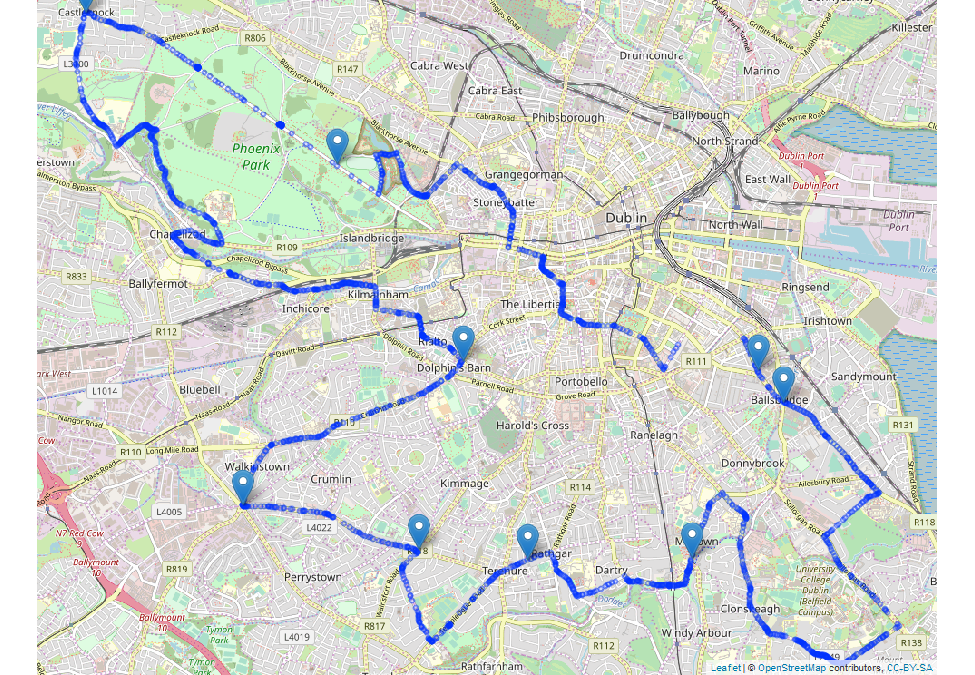
\includegraphics{marathon_cheering_effect_files/figure-latex/cheering-zones-map-1} 

}

\caption{GPS localisation of Cheering Zones on the marathon route.}\label{fig:cheering-zones-map}
\end{figure}

Along the Dublin marathon 2015, eight cheering zones were created
(Figure \ref{fig:cheering-zones-map}). for the purpose of our analysis,
athletes' pace were analysed 1000m before and 1000m after each cheering
zone. However because the two last cheering zones are separated by less
than 1000m, the last cheering zone was not taken into account.

\section{Results}\label{results}

Generalized Linear Models show not only an effect of cheering zones on
atheltes' pace (\(t(5156697) = -2.79\), \(p = .005\)) but also an effect
of the localisation of these cheering zones (\(t(5156697) = -3.84\),
\(p < .001\)) see Table @ref(tab:table\_ischeering).

\begin{table}[tbp]
\begin{center}
\begin{threeparttable}
\caption{\label{tab:table_ischeering}Effect of Cheering Zones according to marathon's route on athletes pace.}
\begin{tabular}{lllll}
\toprule
Predictor & \multicolumn{1}{c}{$b$} & \multicolumn{1}{c}{95\% CI} & \multicolumn{1}{c}{$t(5156697)$} & \multicolumn{1}{c}{$p$}\\
\midrule
Intercept & 5.15 & $[5.15$, $5.16]$ & 3,377.53 & < .001\\
Is cheering1 & -0.13 & $[-0.23$, $-0.04]$ & -2.79 & .005\\
Distance & 0.00 & $[0.00$, $0.00]$ & 481.06 & < .001\\
Is cheering1 $\times$ Distance & 0.00 & $[0.00$, $0.00]$ & -3.84 & < .001\\
\bottomrule
\end{tabular}
\end{threeparttable}
\end{center}
\end{table}

Athletes tend to increase their pace by 0.743\% after each cheering
zones on average but this effect tend to decrease along the marathon
race (Figure \ref{fig:plot-pace-gain}).

\begin{figure}

{\centering 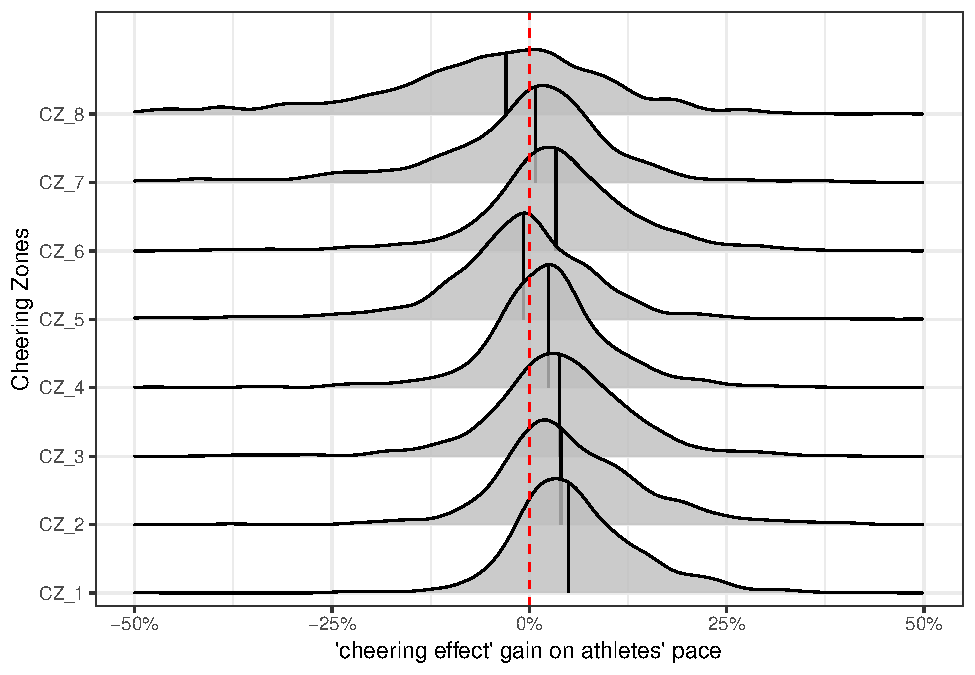
\includegraphics{marathon_cheering_effect_files/figure-latex/plot-pace-gain-1} 

}

\caption{Density distribution of athletes's pace gain during the Cheering Zones.}\label{fig:plot-pace-gain}
\end{figure}

This last result is supported by the comparison athlete's pace
comparison before and after the cheering zones which is significant
overall (\(t(5156695) = 33.44\), \(p < .001\)) and by taken into account
their localisation (\(t(5156695) = -35.18\), \(p < .001\))Table
@ref(tab:table\_before\_after).

\begin{table}[tbp]
\begin{center}
\begin{threeparttable}
\caption{\label{tab:table_before_after}Difference before and after Cheering Zones according to marathon's route on athletes pace.}
\begin{tabular}{lllll}
\toprule
Predictor & \multicolumn{1}{c}{$b$} & \multicolumn{1}{c}{95\% CI} & \multicolumn{1}{c}{$t(5156695)$} & \multicolumn{1}{c}{$p$}\\
\midrule
Intercept & 5.03 & $[5.02$, $5.04]$ & 1,148.40 & < .001\\
Before after0 & 0.13 & $[0.12$, $0.14]$ & 27.03 & < .001\\
Before after1 & 0.21 & $[0.20$, $0.22]$ & 33.44 & < .001\\
Distance & 0.00 & $[0.00$, $0.00]$ & 192.03 & < .001\\
Before after0 $\times$ Distance & 0.00 & $[0.00$, $0.00]$ & -5.39 & < .001\\
Before after1 $\times$ Distance & 0.00 & $[0.00$, $0.00]$ & -35.18 & < .001\\
\bottomrule
\end{tabular}
\end{threeparttable}
\end{center}
\end{table}

\section{Discussion}\label{discussion}

Our results are supporting the theory of individual zones of optimal
functioning (IZOF) for which feeling the support of others in cheering
zones would helps athletes to find the motivation to sublim their
performance (Hagtvet \& Hanin, 2007). Our results are supporting this
idea rather than potential effect of social presence (Lombard \& Ditton,
1997) which would have desappeared once the athletes are out of the
cheering zones (Morgado, Muller, Gentaz, \& Palluel-Germain, 2011).

\newpage

\section{References}\label{references}

\begingroup
\setlength{\parindent}{-0.5in} \setlength{\leftskip}{0.5in}

\hypertarget{refs}{}
\hypertarget{ref-buman2008experiences}{}
Buman, M. P., Omli, J. W., Giacobbi Jr, P. R., \& Brewer, B. W. (2008).
Experiences and coping responses of ``hitting the wall'' for
recreational marathon runners. \emph{Journal of Applied Sport
Psychology}, \emph{20}(3), 282--300.

\hypertarget{ref-hagtvet2007consistency}{}
Hagtvet, K. A., \& Hanin, Y. L. (2007). Consistency of
performance-related emotions in elite athletes: Generalizability theory
applied to the izof model. \emph{Psychology of Sport and Exercise},
\emph{8}(1), 47--72.

\hypertarget{ref-lombard1997heart}{}
Lombard, M., \& Ditton, T. (1997). At the heart of it all: The concept
of presence. \emph{Journal of Computer-Mediated Communication},
\emph{3}(2).

\hypertarget{ref-mccarthy2011positive}{}
McCarthy, P. J. (2011). Positive emotion in sport performance: Current
status and future directions. \emph{International Review of Sport and
Exercise Psychology}, \emph{4}(1), 50--69.

\hypertarget{ref-morgado2011close}{}
Morgado, N., Muller, D., Gentaz, E., \& Palluel-Germain, R. (2011).
Close to me? The influence of affective closeness on space perception.
\emph{Perception}, \emph{40}(7), 877--879.

\hypertarget{ref-shipway2013organisations}{}
Shipway, R., Holloway, I., \& Jones, I. (2013). Organisations,
practices, actors, and events: Exploring inside the distance running
social world. \emph{International Review for the Sociology of Sport},
\emph{48}(3), 259--276.

\hypertarget{ref-vast2010emotions}{}
Vast, R. L., Young, R. L., \& Thomas, P. R. (2010). Emotions in sport:
Perceived effects on attention, concentration, and performance.
\emph{Australian Psychologist}, \emph{45}(2), 132--140.

\endgroup


\end{document}
